\subsection{Carga Electrónica Variable}

Para la realización de los ensayos necesarios para relevar el funcionamiento de la plataforma, se debe contar con algún tipo de carga a la salida del sistema que se encargue de absorber la potencia entregada en la entrada por el emulador de pilas de combustible. Debe ser una carga programable o variable, que permita evaluar el funcionamiento del sistema en las distintas condiciones de carga que se puedan encontrar en un sistema híbrido.\\

El modelo seleccionado para cumplir este rol es la carga programable de corriente continua disponible en el laboratorio, modelo {\Medium IT8514B+} del fabricante ITECH Electronic, que se puede observar en la figura a continuación.\\

\begin{figure}[h]
    \centering
    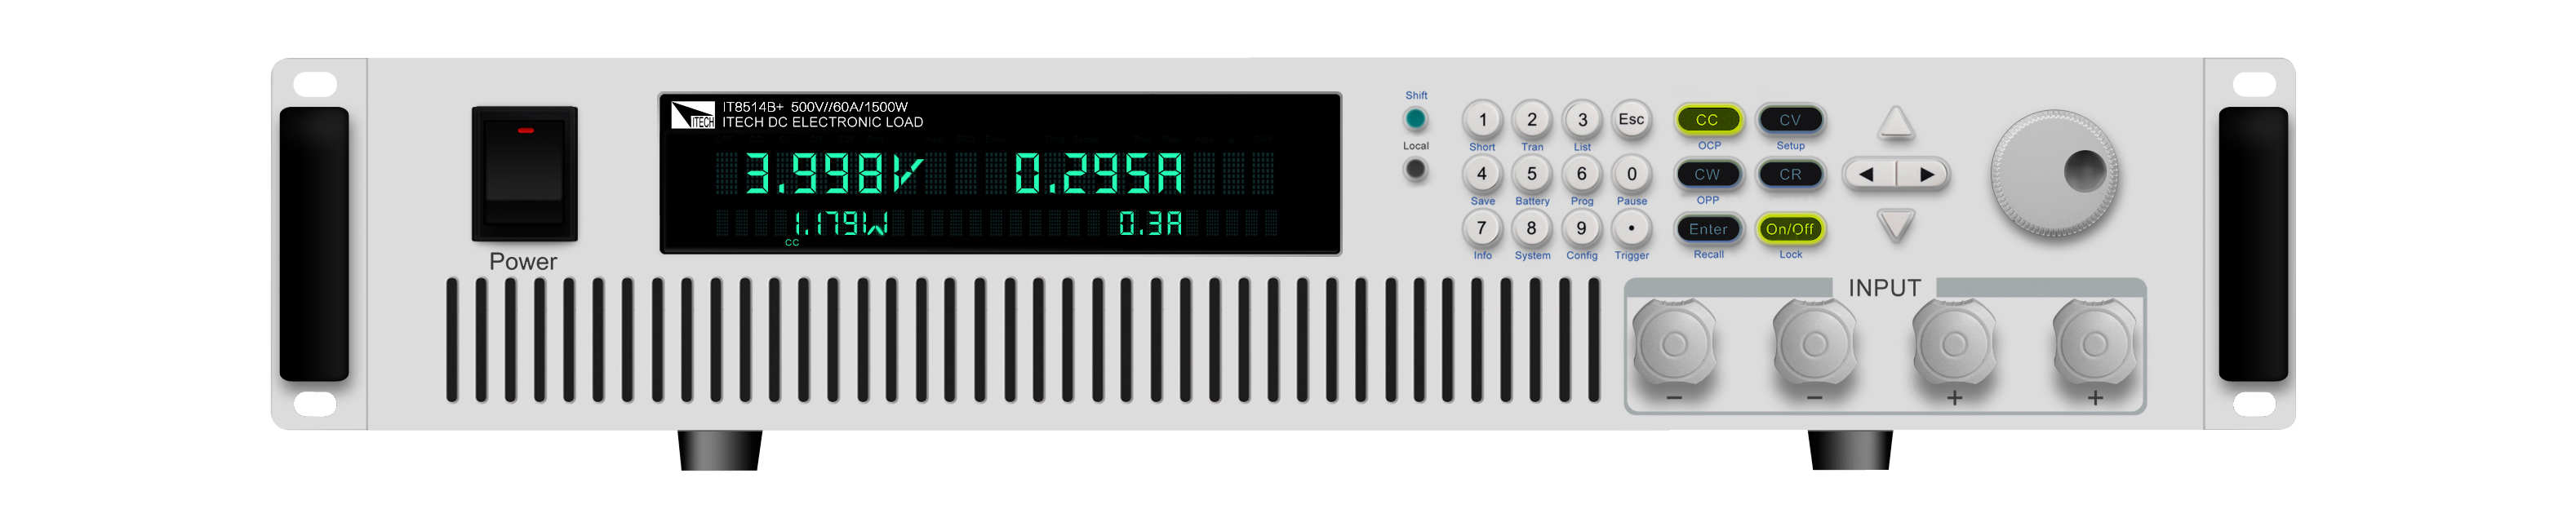
\includegraphics[scale=0.55]{Imagenes/Carga Variable.png}
    \caption{Carga electrónica variable disponible en el laboratorio, modelo ITECH IT8514B+.}
    \label{carga_variable}
\end{figure}

Esta carga programable cuenta con cuatro modos distintos de emulación de carga: corriente constante (CC) hasta \SI[]{60}{\ampere}, tensión constante (CV) hasta \SI[]{500}{\volt}, resistencia constante (CR) y potencia constante (CW) hasta \SI[]{1500}{\watt}. Como se puede ver en la figura \ref{carga_variable}, el dispositivo cuenta con un display en el cuál se indican los valores de tensión, corriente y potencia absorbidos por la carga con alta precisión, evitando la necesidad de utilizar un dispositivo de medida separado para obtener estas figuras.\textsuperscript{\cite{CargaVariable}}\\

Adicionalmente cuenta con modo transitorio, que permite conmutar periódicamente entre dos niveles de carga distintos; y modo de lista, que da la opción de generar una secuencia compleja de niveles de carga, con opciones de sincronización externa e interna.\textsuperscript{\cite{CargaVariable}}\\

Todas estas funcionalidades, junto con su capacidad de tensión, corriente y potencia elevadas, hacen a este un dispositivo ideal para la evaluación del funcionamiento de la plataforma en todas las condiciones de carga necesarias.\\